Consider the following two (valid) class diagrams:

\figureSeriesHere{}{\figureSeriesRow{\figureSeriesElement{1}{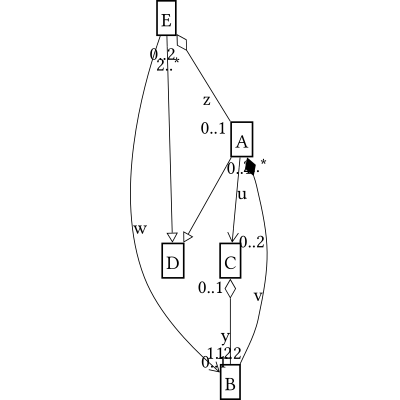
\includegraphics[min width=0.5\textwidth,min height=0.4\textwidth,max width=\textwidth,max height=\textwidth]{57/cdff7492b749b30549ab40da32ad21d9f2cd96dc5d18ebe2847ea5e8674f1fdc1f11af83b04c596701db35357ce8aed00a3a92e08161.pdf}}}\figureSeriesRow{\figureSeriesElement{2}{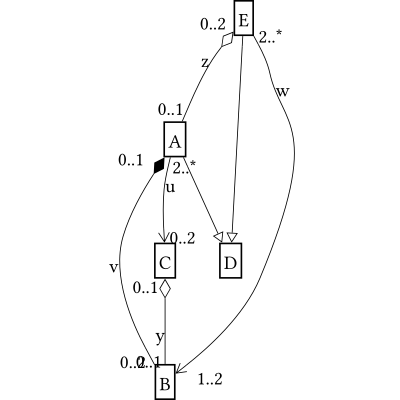
\includegraphics[min width=0.5\textwidth,min height=0.4\textwidth,max width=\textwidth,max height=\textwidth]{57/cdef10df18fc6a9b17b7b686f5107f2ee2484ec1dd93bc41ed450de47e6375d42f11af83b04c596701db35357ce8aed00a3a92e08161.pdf}}}}Which of the following five object diagrams conform to which class diagram? 
 An object diagram can conform to neither, either, or both class diagrams.

\figureSeriesHere{}{\figureSeriesRow{\figureSeriesElement{a}{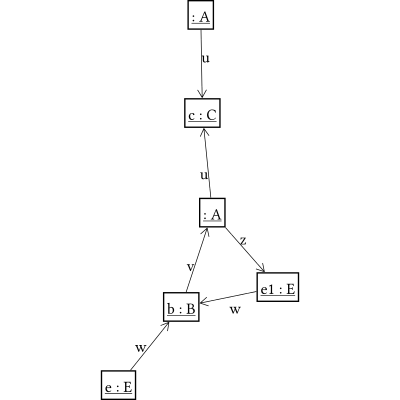
\includegraphics[min width=0.5\textwidth,min height=0.4\textwidth,max width=\textwidth,max height=\textwidth]{57/ode57aa5469f9f2dd44368aa91178979b8f103341a7f930a3279bfafb1bb30c0f010.pdf}}}\figureSeriesRow{\figureSeriesElement{b}{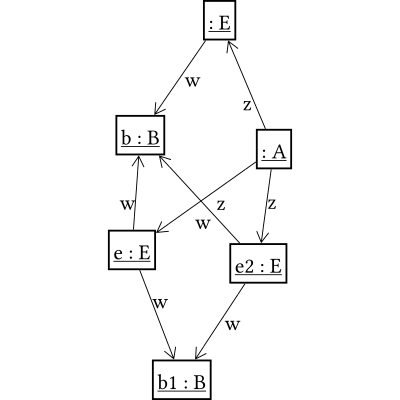
\includegraphics[min width=0.5\textwidth,min height=0.4\textwidth,max width=\textwidth,max height=\textwidth]{57/od75f9c60a674815df61364525868bb7fd7223554a2ba69b8d6a193f7d818a9ad410.pdf}}}\figureSeriesRow{\figureSeriesElement{c}{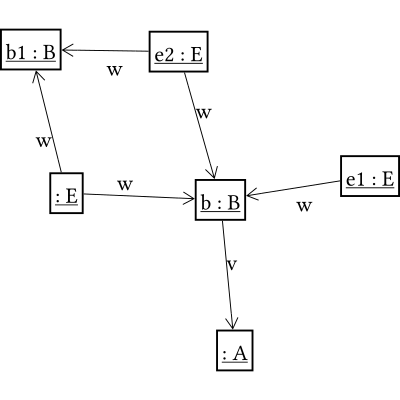
\includegraphics[min width=0.5\textwidth,min height=0.4\textwidth,max width=\textwidth,max height=\textwidth]{57/od048acd84abd07c0b546c9fc19f7fc92b0dbbfe344a19127858530926e742d25710.pdf}}}\figureSeriesRow{\figureSeriesElement{d}{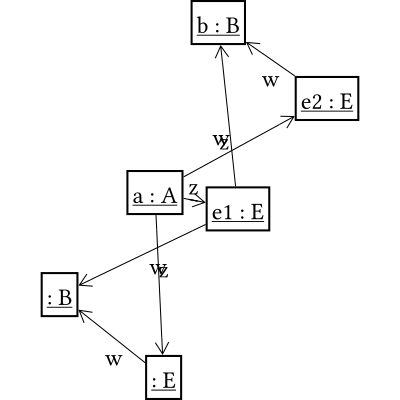
\includegraphics[min width=0.5\textwidth,min height=0.4\textwidth,max width=\textwidth,max height=\textwidth]{57/od011c35c5ebab841204649ea8afb7dbcd6fd4a656695175ce7f24d7ecef364e3c10.pdf}}}\figureSeriesRow{\figureSeriesElement{e}{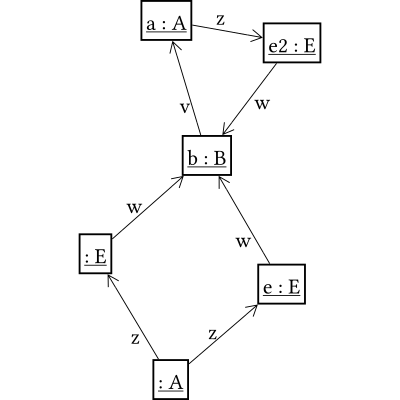
\includegraphics[min width=0.5\textwidth,min height=0.4\textwidth,max width=\textwidth,max height=\textwidth]{57/od08d8ec553b02600176e3e5a4cd1470a440e102a8093e9ba94706978c600abb4e10.pdf}}}}Please state your answer by giving a list of pairs, each comprising of a class diagram number and object diagram letters. 
 Each pair indicates that the mentioned object diagrams conform to the respective class diagram. 
 For example, 
\begin{minted}{text}
[(1,ab),(2,)]
\end{minted}
expresses that among the offered choices exactly the object diagrams a and b are instances of class diagram 1 and that none of the offered object diagrams are instances of class diagram 2.

Please note: Classes are represented simplified here. 
 That means they consist of a single box containing only the class name but no sections for attributes or methods. 
 Nevertheless you should treat these simplified class representations as valid classes.

As navigation directions are used, please note that aggregations and compositions are only navigable from the ``part'' toward the ``whole'', i.e., they are not navigable in the opposite direction!

Please note: When hovering over or clicking on edges / nodes or their labels, the respective components that belong together are highlighted.

